\documentclass[14pt]{extbook}
\usepackage{multicol, enumerate, enumitem, hyperref, color, soul, setspace, parskip, fancyhdr} %General Packages
\usepackage{amssymb, amsthm, amsmath, latexsym, units, mathtools} %Math Packages
\everymath{\displaystyle} %All math in Display Style
% Packages with additional options
\usepackage[headsep=0.5cm,headheight=12pt, left=1 in,right= 1 in,top= 1 in,bottom= 1 in]{geometry}
\usepackage[usenames,dvipsnames]{xcolor}
\usepackage{dashrule}  % Package to use the command below to create lines between items
\newcommand{\litem}[1]{\item#1\hspace*{-1cm}\rule{\textwidth}{0.4pt}}
\pagestyle{fancy}
\lhead{Progress Quiz 5}
\chead{}
\rhead{Version B}
\lfoot{8497-6012}
\cfoot{}
\rfoot{Summer C 2021}
\begin{document}

\begin{enumerate}
\litem{
Construct the lowest-degree polynomial given the zeros below. Then, choose the intervals that contain the coefficients of the polynomial in the form $x^3+bx^2+cx+d$.\[ -5 + 4 i \text{ and } 1 \]\begin{enumerate}[label=\Alph*.]
\item \( b \in [7, 12], c \in [31, 38], \text{ and } d \in [-48, -38] \)
\item \( b \in [0, 5], c \in [-2, 10], \text{ and } d \in [-10, -2] \)
\item \( b \in [-10, -7], c \in [31, 38], \text{ and } d \in [35, 42] \)
\item \( b \in [0, 5], c \in [-7, 0], \text{ and } d \in [2, 5] \)
\item \( \text{None of the above.} \)

\end{enumerate} }
\litem{
Construct the lowest-degree polynomial given the zeros below. Then, choose the intervals that contain the coefficients of the polynomial in the form $ax^3+bx^2+cx+d$.\[ \frac{-7}{3}, \frac{-3}{2}, \text{ and } -1 \]\begin{enumerate}[label=\Alph*.]
\item \( a \in [0, 8], b \in [-18, -13], c \in [-7, -1], \text{ and } d \in [20, 27] \)
\item \( a \in [0, 8], b \in [-31, -26], c \in [43, 48], \text{ and } d \in [-21, -18] \)
\item \( a \in [0, 8], b \in [-2, 12], c \in [-29, -22], \text{ and } d \in [-21, -18] \)
\item \( a \in [0, 8], b \in [26, 34], c \in [43, 48], \text{ and } d \in [-21, -18] \)
\item \( a \in [0, 8], b \in [26, 34], c \in [43, 48], \text{ and } d \in [20, 27] \)

\end{enumerate} }
\litem{
Describe the end behavior of the polynomial below.\[ f(x) = 8(x + 3)^{5}(x - 3)^{10}(x + 9)^{2}(x - 9)^{3} \]\begin{enumerate}[label=\Alph*.]
\begin{multicols}{2}\item 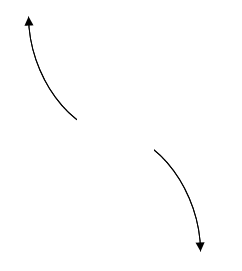
\includegraphics[width = 0.3\textwidth]{../Figures/polyEndBehaviorAB.png}\item 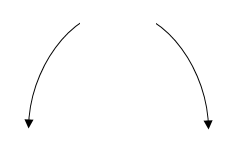
\includegraphics[width = 0.3\textwidth]{../Figures/polyEndBehaviorBB.png}\item 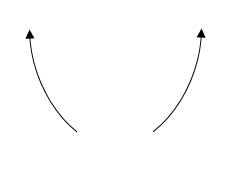
\includegraphics[width = 0.3\textwidth]{../Figures/polyEndBehaviorCB.png}\item 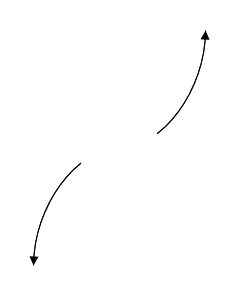
\includegraphics[width = 0.3\textwidth]{../Figures/polyEndBehaviorDB.png}\end{multicols}\item None of the above.
\end{enumerate} }
\litem{
Which of the following equations \textit{could} be of the graph presented below?
\begin{center}
    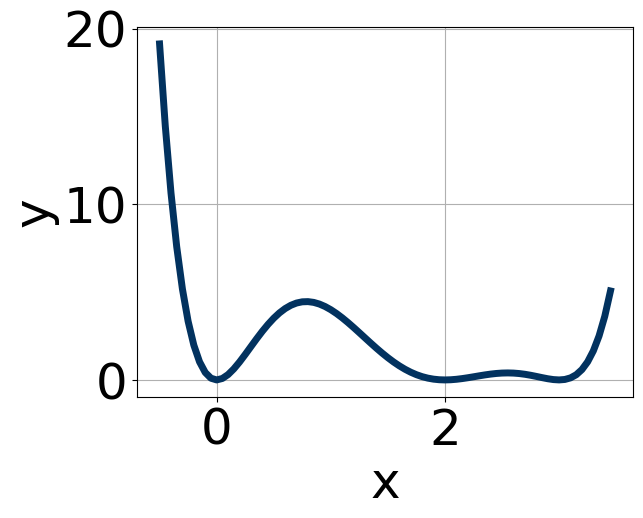
\includegraphics[width=0.5\textwidth]{../Figures/polyGraphToFunctionCopyB.png}
\end{center}
\begin{enumerate}[label=\Alph*.]
\item \( -6x^{10} (x - 3)^{8} (x - 2)^{11} \)
\item \( -12x^{8} (x - 3)^{10} (x - 2)^{10} \)
\item \( 20x^{8} (x - 3)^{4} (x - 2)^{6} \)
\item \( 19x^{10} (x - 3)^{10} (x - 2)^{5} \)
\item \( 17x^{7} (x - 3)^{8} (x - 2)^{7} \)

\end{enumerate} }
\litem{
Construct the lowest-degree polynomial given the zeros below. Then, choose the intervals that contain the coefficients of the polynomial in the form $ax^3+bx^2+cx+d$.\[ \frac{-3}{4}, 4, \text{ and } \frac{4}{3} \]\begin{enumerate}[label=\Alph*.]
\item \( a \in [6, 19], b \in [54, 56], c \in [13, 20], \text{ and } d \in [-52, -44] \)
\item \( a \in [6, 19], b \in [-58, -53], c \in [13, 20], \text{ and } d \in [-52, -44] \)
\item \( a \in [6, 19], b \in [-58, -53], c \in [13, 20], \text{ and } d \in [47, 52] \)
\item \( a \in [6, 19], b \in [22, 29], c \in [-90, -84], \text{ and } d \in [47, 52] \)
\item \( a \in [6, 19], b \in [-77, -65], c \in [111, 121], \text{ and } d \in [-52, -44] \)

\end{enumerate} }
\litem{
Which of the following equations \textit{could} be of the graph presented below?
\begin{center}
    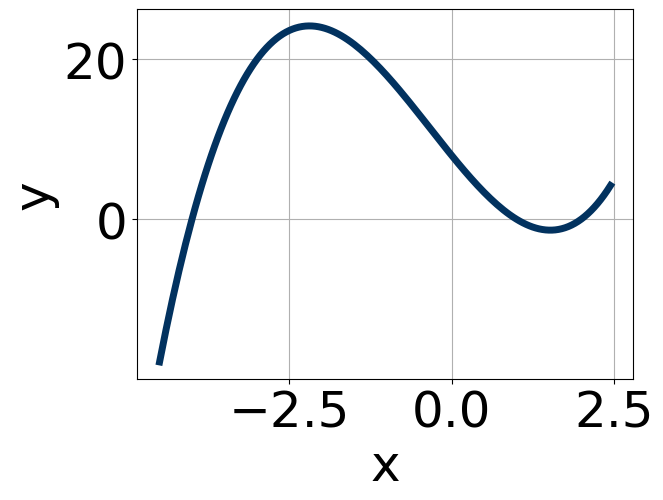
\includegraphics[width=0.5\textwidth]{../Figures/polyGraphToFunctionB.png}
\end{center}
\begin{enumerate}[label=\Alph*.]
\item \( -7(x - 1)^{8} (x - 2)^{7} (x + 4)^{11} \)
\item \( -17(x - 1)^{5} (x - 2)^{9} (x + 4)^{9} \)
\item \( 11(x - 1)^{7} (x - 2)^{9} (x + 4)^{7} \)
\item \( 20(x - 1)^{10} (x - 2)^{8} (x + 4)^{11} \)
\item \( 18(x - 1)^{6} (x - 2)^{11} (x + 4)^{5} \)

\end{enumerate} }
\litem{
Describe the zero behavior of the zero $x = -4$ of the polynomial below.\[ f(x) = 4(x + 4)^{8}(x - 4)^{13}(x - 8)^{2}(x + 8)^{6} \]\begin{enumerate}[label=\Alph*.]
\begin{multicols}{2}\item 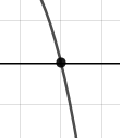
\includegraphics[width = 0.3\textwidth]{../Figures/polyZeroBehaviorAB.png}\item 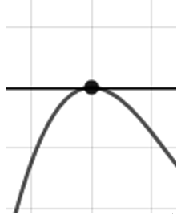
\includegraphics[width = 0.3\textwidth]{../Figures/polyZeroBehaviorBB.png}\item 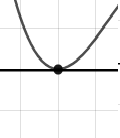
\includegraphics[width = 0.3\textwidth]{../Figures/polyZeroBehaviorCB.png}\item 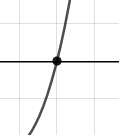
\includegraphics[width = 0.3\textwidth]{../Figures/polyZeroBehaviorDB.png}\end{multicols}\item None of the above.
\end{enumerate} }
\litem{
Describe the zero behavior of the zero $x = -6$ of the polynomial below.\[ f(x) = -4(x - 8)^{12}(x + 8)^{8}(x + 6)^{11}(x - 6)^{8} \]\begin{enumerate}[label=\Alph*.]
\begin{multicols}{2}\item 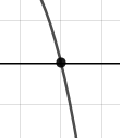
\includegraphics[width = 0.3\textwidth]{../Figures/polyZeroBehaviorCopyAB.png}\item 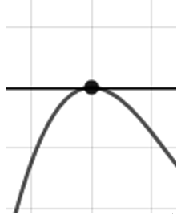
\includegraphics[width = 0.3\textwidth]{../Figures/polyZeroBehaviorCopyBB.png}\item 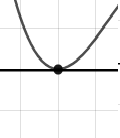
\includegraphics[width = 0.3\textwidth]{../Figures/polyZeroBehaviorCopyCB.png}\item 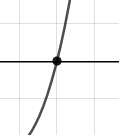
\includegraphics[width = 0.3\textwidth]{../Figures/polyZeroBehaviorCopyDB.png}\end{multicols}\item None of the above.
\end{enumerate} }
\litem{
Construct the lowest-degree polynomial given the zeros below. Then, choose the intervals that contain the coefficients of the polynomial in the form $x^3+bx^2+cx+d$.\[ -5 + 4 i \text{ and } 4 \]\begin{enumerate}[label=\Alph*.]
\item \( b \in [-7.2, -3.1], c \in [-6, 9], \text{ and } d \in [157, 173] \)
\item \( b \in [-1.8, 4.3], c \in [-6, 9], \text{ and } d \in [-26, -16] \)
\item \( b \in [-1.8, 4.3], c \in [-10, -5], \text{ and } d \in [16, 23] \)
\item \( b \in [5.4, 7.5], c \in [-6, 9], \text{ and } d \in [-165, -163] \)
\item \( \text{None of the above.} \)

\end{enumerate} }
\litem{
Describe the end behavior of the polynomial below.\[ f(x) = 4(x - 9)^{3}(x + 9)^{8}(x - 8)^{4}(x + 8)^{4} \]\begin{enumerate}[label=\Alph*.]
\begin{multicols}{2}\item 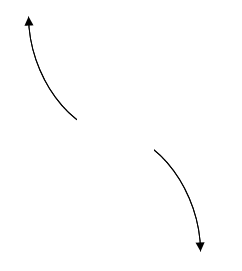
\includegraphics[width = 0.3\textwidth]{../Figures/polyEndBehaviorCopyAB.png}\item 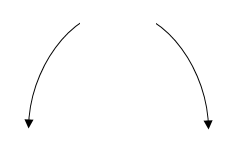
\includegraphics[width = 0.3\textwidth]{../Figures/polyEndBehaviorCopyBB.png}\item 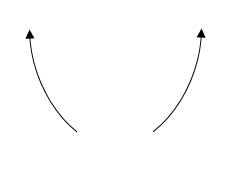
\includegraphics[width = 0.3\textwidth]{../Figures/polyEndBehaviorCopyCB.png}\item 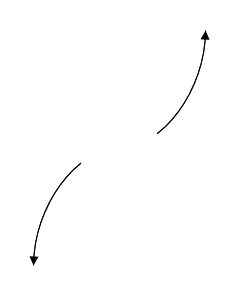
\includegraphics[width = 0.3\textwidth]{../Figures/polyEndBehaviorCopyDB.png}\end{multicols}\item None of the above.
\end{enumerate} }
\end{enumerate}

\end{document}